%%%%%%%%%%%%%%%%%%%%%%%%%%%%%%%%%%%%%%%%%
% Beamer Presentation
% LaTeX Template
% Version 1.0 (10/11/12)
%
% This template has been downloaded from:
% http://www.LaTeXTemplates.com
%
% License:
% CC BY-NC-SA 3.0 (http://creativecommons.org/licenses/by-nc-sa/3.0/)
%
%%%%%%%%%%%%%%%%%%%%%%%%%%%%%%%%%%%%%%%%%

%----------------------------------------------------------------------------------------
%	PACKAGES AND THEMES
%----------------------------------------------------------------------------------------

\documentclass{beamer}

\mode<presentation> {

% The Beamer class comes with a number of default slide themes
% which change the colors and layouts of slides. Below this is a list
% of all the themes, uncomment each in turn to see what they look like.

%\usetheme{default}
%\usetheme{AnnArbor}
%\usetheme{Antibes}
%\usetheme{Bergen}
%\usetheme{Berkeley}
%\usetheme{Berlin}
%\usetheme{Boadilla}
%\usetheme{CambridgeUS}
%\usetheme{Copenhagen}
%\usetheme{Darmstadt}
%\usetheme{Dresden}
%\usetheme{Frankfurt}
%\usetheme{Goettingen}
%\usetheme{Hannover}
%\usetheme{Ilmenau}
%\usetheme{JuanLesPins}
%\usetheme{Luebeck}
\usetheme{Madrid}
%\usetheme{Malmoe}
%\usetheme{Marburg}
%\usetheme{Montpellier}
%\usetheme{PaloAlto}
%\usetheme{Pittsburgh}
%\usetheme{Rochester}
%\usetheme{Singapore}
%\usetheme{Szeged}
%\usetheme{Warsaw}

% As well as themes, the Beamer class has a number of color themes
% for any slide theme. Uncomment each of these in turn to see how it
% changes the colors of your current slide theme.

%\usecolortheme{albatross}
%\usecolortheme{beaver}
%\usecolortheme{beetle}
%\usecolortheme{crane}
%\usecolortheme{dolphin}
%\usecolortheme{dove}
%\usecolortheme{fly}
%\usecolortheme{lily}
%\usecolortheme{orchid}
%\usecolortheme{rose}
%\usecolortheme{seagull}
%\usecolortheme{seahorse}
%\usecolortheme{whale}
%\usecolortheme{wolverine}

%\setbeamertemplate{footline} % To remove the footer line in all slides uncomment this line
%\setbeamertemplate{footline}[page number] % To replace the footer line in all slides with a simple slide count uncomment this line

%\setbeamertemplate{navigation symbols}{} % To remove the navigation symbols from the bottom of all slides uncomment this line
}
\usepackage[utf8]{inputenc}
\usepackage[T1]{fontenc}
\usepackage[brazilian]{babel}
\usepackage{graphicx} % Allows including images
\usepackage{booktabs} % Allows the use of \toprule, \midrule and \bottomrule in tables
\usepackage{caption}

%----------------------------------------------------------------------------------------
%	TITLE PAGE
%----------------------------------------------------------------------------------------

\title[Short title]{Breast Cancer Wisconsin (Diagnostic)} % The short title appears at the bottom of every slide, the full title is only on the title page

\author{Luís Gustavo \\
Aramys Almeida Matos
} % Your name

\institute[UFRJ] % Your institution as it will appear on the bottom of every slide, may be shorthand to save space
{
Inteligência Computacional \\ % Your institution for the title page
\medskip
%\textit{john@smith.com} % Your email address
}
\date{\today} % Date, can be changed to a custom date

\begin{document}

\begin{frame}
\titlepage % Print the title page as the first slide
\end{frame}

%\begin{frame}
%%\frametitle{Overview} % Table of contents slide, comment this block out to remove it
%\tableofcontents % Throughout your presentation, if you choose to use \section{} and \subsection{} commands, these will automatically be printed on this slide as an overview of your presentation
%\end{frame}

%----------------------------------------------------------------------------------------
%	PRESENTATION SLIDES
%----------------------------------------------------------------------------------------

%------------------------------------------------
\section{First Section} % Sections can be created in order to organize your presentation into discrete blocks, all sections and subsections are automatically printed in the table of contents as an overview of the talk
%------------------------------------------------

\subsection{Subsection Example} % A subsection can be created just before a set of slides with a common theme to further break down your presentation into chunks

\begin{frame}
\frametitle{Dataset}
\begin{itemize}
\item Exames para câncer de mama.
\item Características do núcleo de células computadas a partir de imagens digitalizadas
\item 30 variáveis de entrada
\item 1 variável de saída
\item Raio, textura, perímetro, área, suavidade, compacidade, concavidade, pontos côncavos, simetria, dimensão fractal
\end{itemize}
\end{frame}

\begin{frame}
\frametitle{Problema}
\begin{itemize}
\item Problema de classificação
\item Identificar se o câncer é benigno ou maligno.
\item Aplicar e avaliar os modelos de classificação:
\begin{itemize}
\item Classificador Bayesiano Simples
\item Classificador Bayesiano Quadrático
\item Regressão Logística
\item Perceptron
\item Perceptron Múltiplas Camadas
\end{itemize}
\end{itemize}
\end{frame}


%------------------------------------------------

\begin{frame}
\frametitle{Matriz de Correlação}
\begin{figure}[H]
    \centering
    %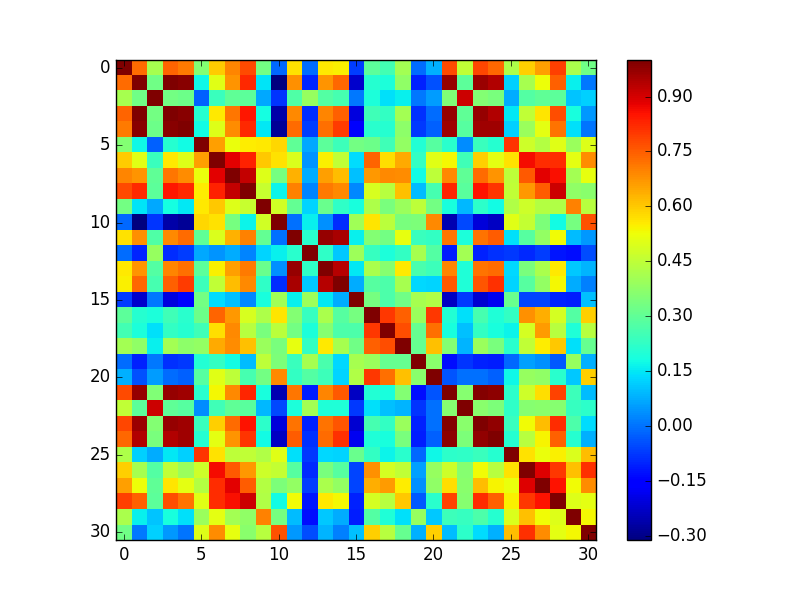
\includegraphics[width=0.8\textwidth]{../corrcoef.png}
    \label{fig:corrcoef}
\end{figure}
\end{frame}

%------------------------------------------------

\begin{frame}
\frametitle{Distância Euclidiana}
\begin{figure}[H]
    \centering
    %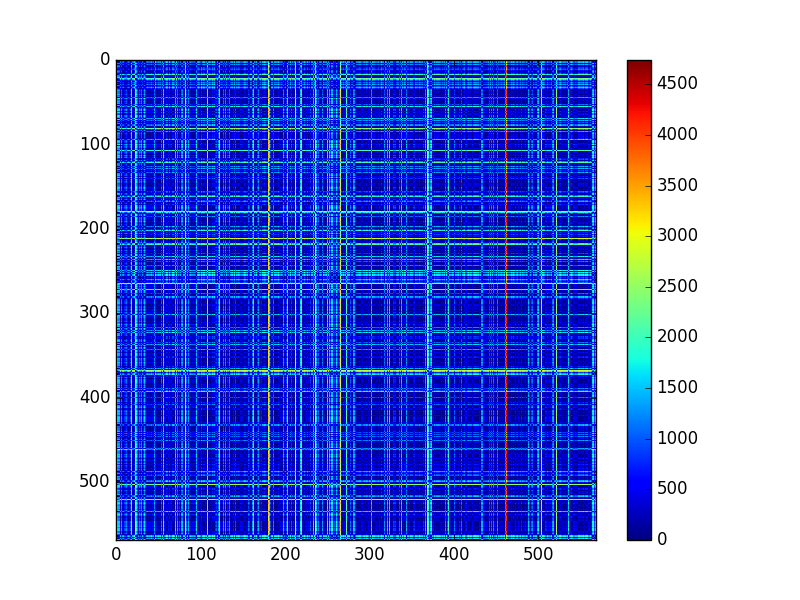
\includegraphics[width=0.8\textwidth]{../dist.png}
    \label{fig:corrcoef}
\end{figure}
\end{frame}
%------------------------------------------------

\begin{frame}

\frametitle{Histogramas}
Smoothness
\begin{figure}[H]
\centering
  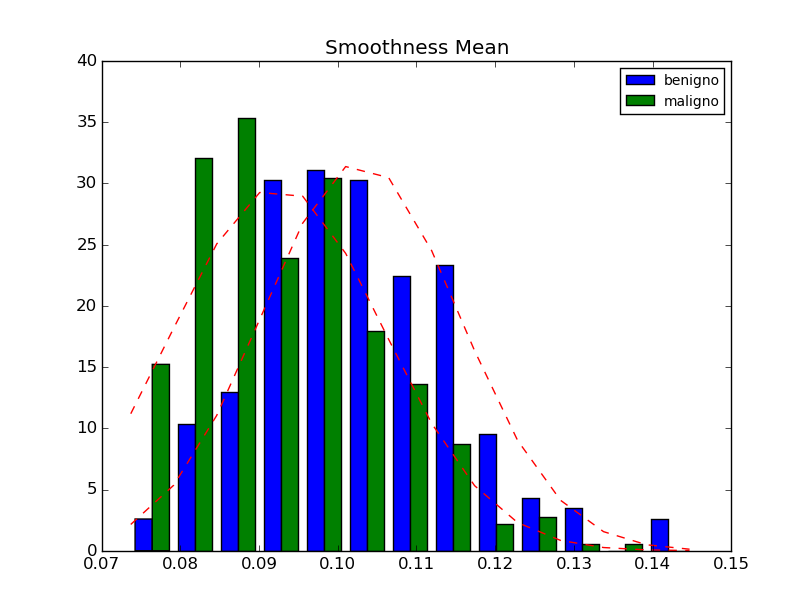
\includegraphics[width=.3\linewidth]{./Histogramas/Smoothness_Mean}
  %\captionof{figure}{Mean}
  \label{fig:test1}
\end{figure}%

\begin{figure}[H]
\centering
\begin{minipage}{.3\textwidth}
  \centering
  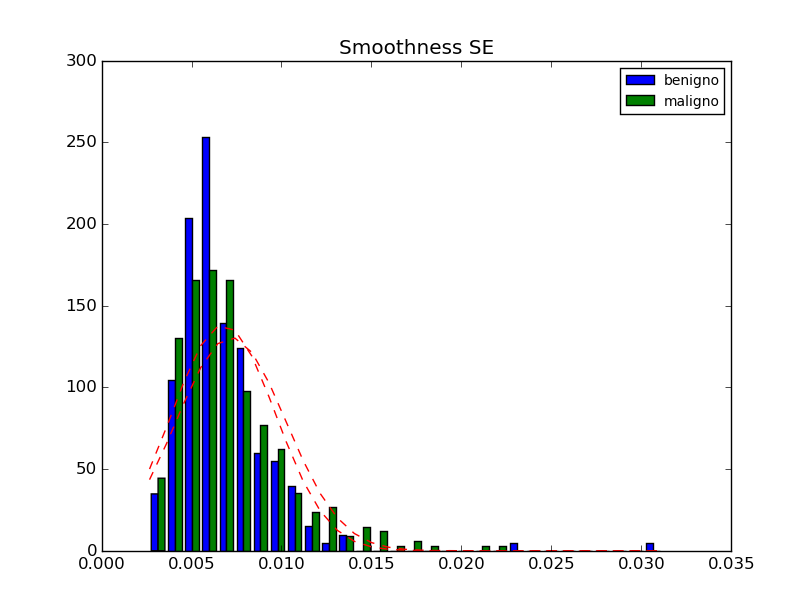
\includegraphics[width=\linewidth]{./Histogramas/Smoothness_SE}
  %\captionof{figure}{Standard Error}
  \label{fig:test1}
\end{minipage}%
\begin{minipage}{.3\textwidth}
  \centering
  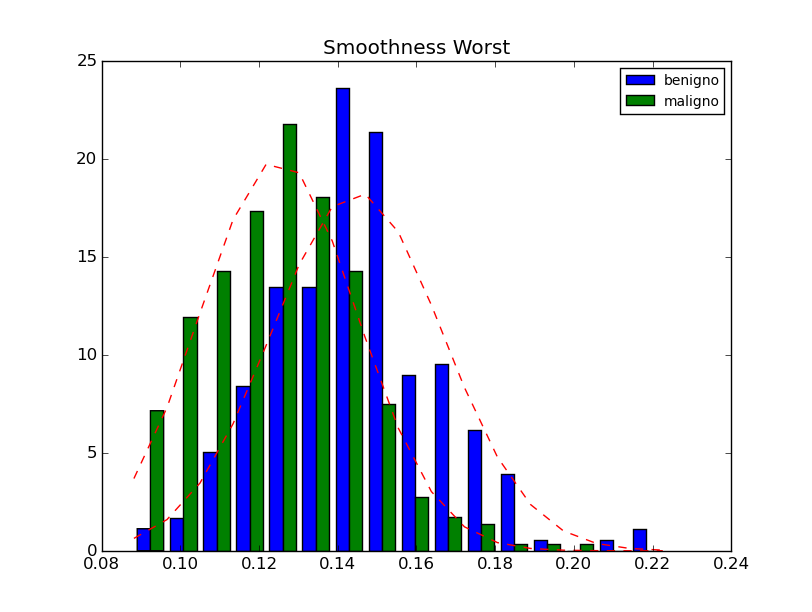
\includegraphics[width=\linewidth]{./Histogramas/Smoothness_Worst}
  %\captionof{figure}{Worst}
  \label{fig:test2}
\end{minipage}
\end{figure}

\end{frame}

\begin{frame}
\frametitle{Histogramas}
Texture
\begin{figure}[H]
\centering
  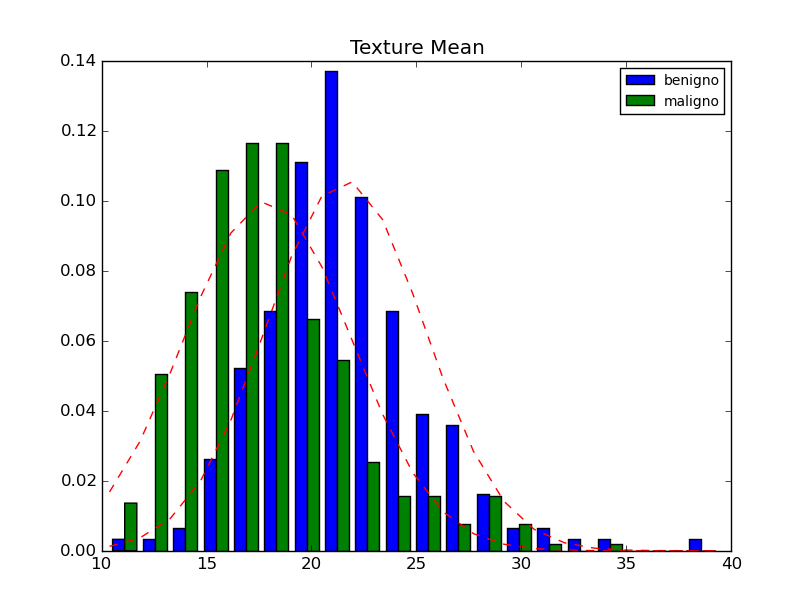
\includegraphics[width=.3\linewidth]{./Histogramas/Texture_Mean}
  %\captionof{figure}{Mean}
  \label{fig:test1}
\end{figure}%

\begin{figure}[H]
\centering
\begin{minipage}{.3\textwidth}
  \centering
  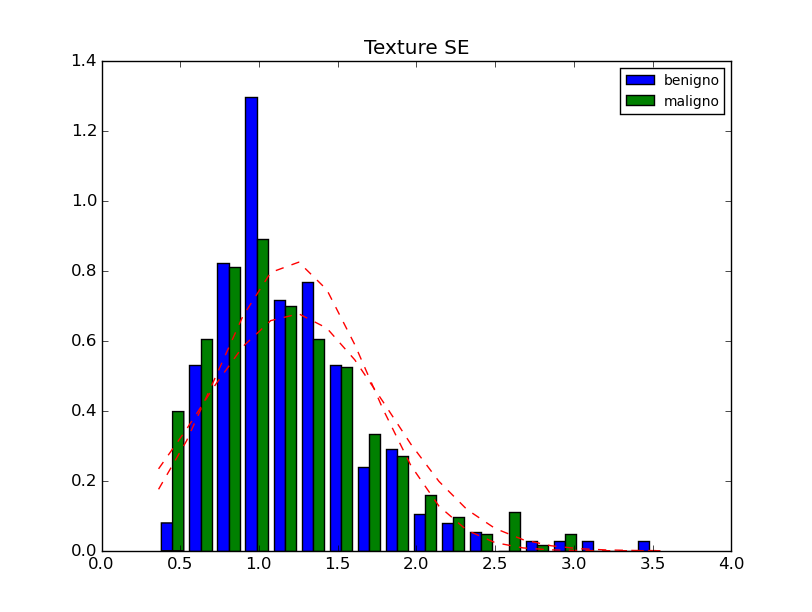
\includegraphics[width=\linewidth]{./Histogramas/Texture_SE}
  %\captionof{figure}{Standard Error}
  \label{fig:test1}
\end{minipage}%
\begin{minipage}{.3\textwidth}
  \centering
  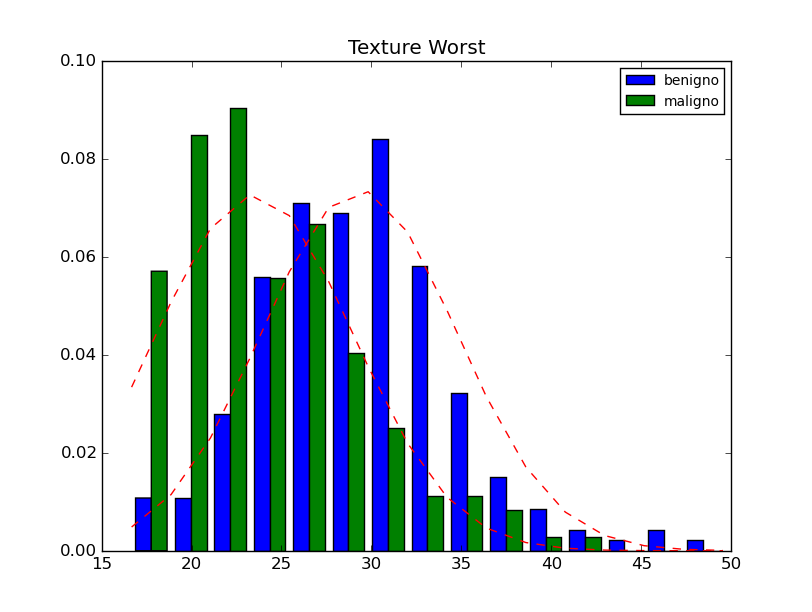
\includegraphics[width=\linewidth]{./Histogramas/Texture_Worst}
  %\captionof{figure}{Worst}
  \label{fig:test2}
\end{minipage}
\end{figure}
\end{frame}
%------------------------------------------------


\begin{frame}
\frametitle{Tecnologia}
\begin{block}{Python}
\begin{itemize}
\item SciPy
	\begin{itemize}
	\item \textit{NumPy}
	\item \textit{matplotlib}
	\item \textit{pandas}: Python Data Analysis Library
	\end{itemize}
\item \textit{scikit-learn}: Machine Learning in Python
\end{itemize}
\end{block}

\begin{block}{Matlab}
\begin{itemize}
\item Statistics and Machine Learning Toolbox
\end{itemize}
\end{block}

\end{frame}


\begin{frame}
\frametitle{Metodologia}
Para cada método de classificação foi feito:
\begin{itemize}
\item Validação cruzada de 10 ciclos
\item Matriz de confusão (média de cada ciclo)
\item Métricas de acurácia, precisão, recuperão. 
\end{itemize}
\end{frame}


\begin{frame}
\frametitle{Classificador Bayesiano Simples (Naive Bayes)}
\begin{itemize} 
\item Aplicação do teorema de Bayes
\item Supoe que cada par de variáveis é independente
\end{itemize}

\begin{theorem}[Teorema de Bayes]
\[P(y|x_1 \dots x_n)  = \frac{P(y)P(x_1, \dots, x_n|y)}{P(x_1,\dots, x_n)}\]
Onde:

$y$ é a variável de saída que identifica a classe

$x = [x_1, \dots, x_n] $ é o vetor de entrada 

\end{theorem}

\end{frame}

\begin{frame}
\frametitle{Classificador Bayesiano (Naive Bayes) - Resultados}

\textbf{Avaliação dos resultados}
\begin{columns}[c] 
\column{.45\textwidth} % Left column and width
\begin{itemize}
\item ACC = 0.94
\end{itemize}

\begin{table}
\begin{tabular}{l l l}
\toprule
 & \textbf{$\hat{C}_1$ (Predita)} & \textbf{$\hat{C}_2$(Predita)}\\
\midrule
$C_1$ & 18.80&2.40\\ 
$C_2$ &  1.20&34.50\\ 
\bottomrule
\end{tabular}
\caption{Matriz de confusão}
\end{table}


\column{.5\textwidth} % Right column and width
\begin{figure}[H]
\centering
  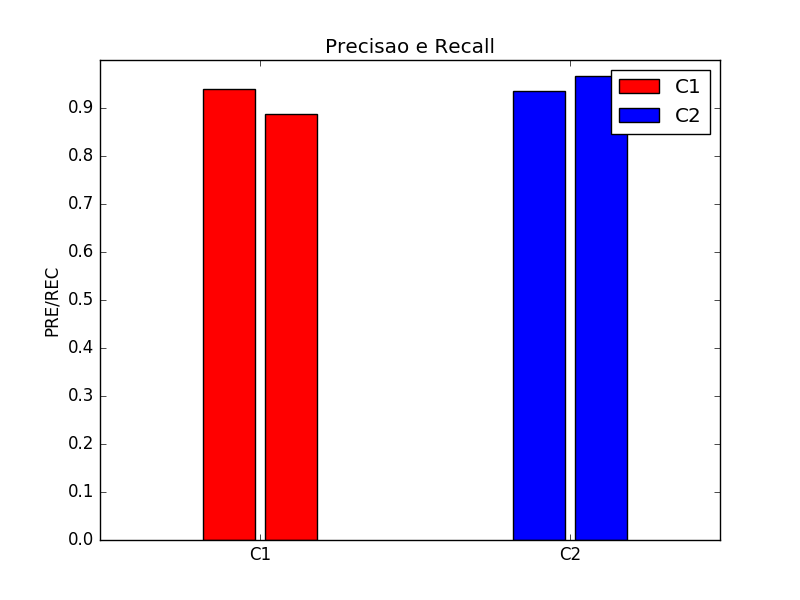
\includegraphics[width=\linewidth]{../img/naive_bayes_rec.png}
  \captionof{figure}{Precisão e Recall}
  \label{fig:percep}
\end{figure}%

\end{columns}

\end{frame}



\begin{frame}
\frametitle{Classificador Bayesiano Quadrático}
\begin{itemize} 
\item Um classificador com uma fronteira de decisão quadrática, gerado pela densidades condicionais dos dados e utilizando a regra de Bayes.
\item A decisão é calculada pela função discriminante:
\end{itemize}

\begin{theorem}[Função Discriminante]
\[ g_i(x(t))= ln P(C_i|x(t))= ln p(x(t)|C_i)+ ln P(C_i)\]

\end{theorem}

\end{frame}

\begin{frame}
\frametitle{Classificador Bayesiano Quadrático - Resultados}

\textbf{Avaliação dos resultados}
\begin{columns}[c] 
\column{.45\textwidth} % Left column and width
\begin{itemize}
\item ACC = 0.96
\end{itemize}

\begin{table}
\begin{tabular}{l l l}
\toprule
 & \textbf{$\hat{C}_1$ (Predita)} & \textbf{$\hat{C}_2$(Predita)}\\
\midrule
$C_1$ & 20.00&1.20\\ 
$C_2$ &  1.20&34.50\\ 

\bottomrule
\end{tabular}
\caption{Matriz de confusão}
\end{table}


\column{.5\textwidth} % Right column and width
\begin{figure}[H]
\centering
  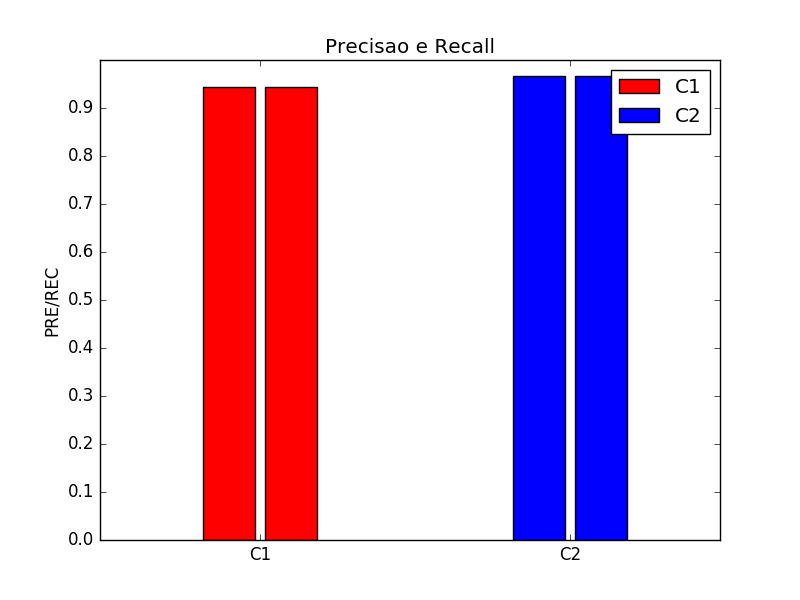
\includegraphics[width=\linewidth]{../img/quad_bayes_rec.png}
  \captionof{figure}{Precisão e Recall}
  \label{fig:percep}
\end{figure}%

\end{columns}

\end{frame}




\begin{frame}
\frametitle{Regessão Logística}
\begin{itemize} 
\item Na regressão logística, a saída do modelo é uma aproximação da
probabilidade a posteriori.
\item A função discriminante é calculada pela função sigmoide, ou função logística ou logit
\end{itemize}

\begin{theorem}[Função Logística]
\[g_i(x(t)|\theta_i))  = \frac{1}{1+ exp(\hat{x}(t)\theta_i)}\]
Onde:
\[\hat{x}(t) = [1,x(t)] e \theta_i=[\theta\textsubscript{i0},\theta\textsubscript{i1}]^T\]

\end{theorem}

\end{frame}

\begin{frame}
\frametitle{Regessão Logística - Resultados}

\textbf{Avaliação dos resultados}
\begin{columns}[c] 
\column{.45\textwidth} % Left column and width
\begin{itemize}
\item ACC = 0.96
\end{itemize}

\begin{table}
\begin{tabular}{l l l}
\toprule
 & \textbf{$\hat{C}_1$ (Predita)} & \textbf{$\hat{C}_2$(Predita)}\\
\midrule
$C_1$ & 20.00&1.20\\ 
$C_2$ & 1.10&34.60\\ 

\bottomrule
\end{tabular}
\caption{Matriz de confusão}
\end{table}


\column{.5\textwidth} % Right column and width
\begin{figure}[H]
\centering
  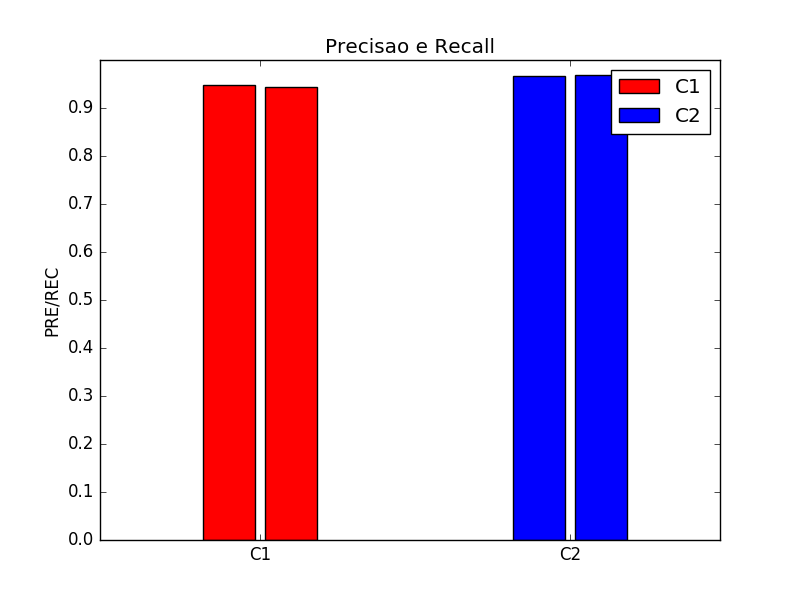
\includegraphics[width=\linewidth]{../img/log_reg_rec.png}
  \captionof{figure}{Precisão e Recall}
  \label{fig:percep}
\end{figure}%

\end{columns}

\end{frame}





\begin{frame}
\frametitle{Perceptron}
O Perceptron utiliza o modelo McCulloch-Pitts para o neurônio artificial. O processamento de cada unidade é dado por:
\begin{block}{McCulloch-Pitts}
\[ u(t) = h(z(t)) = h \left( \theta_0 + \sum_{i=1}^n x_i(t) \theta_i \right) \]
Onde:

$u(t)$: valor de ativação

$z(t)$: potencial de ativaçãos

$h$: função de ativação

$x_i(t)$: entradas do neurônio
\end{block}
\end{frame}


\begin{frame}[fragile] % Need to use the fragile option when verbatim is used in the slide
\frametitle{Perceptron - Implementação}
\begin{block}{Scikit Learn}
\begin{verbatim}
class sklearn.linear_model.Perceptron(penalty=None, 
  alpha=0.0001, fit_intercept=True, n_iter=5, 
  shuffle=True, verbose=0, eta0=1.0, n_jobs=1, 
  random_state=0, class_weight=None, warm_start=False)
\end{verbatim}
\end{block}
É uma expecialização do \verb|sklearn.linear_model.SGDClassifier|.
\end{frame}

\begin{frame}
\frametitle{Perceptron - Resultados}
\textbf{Avaliação dos resultados}
\begin{columns}[c] 
\column{.45\textwidth} % Left column and width
\begin{itemize}
\item ACC = 0.96
\end{itemize}

\begin{table}
\begin{tabular}{l l l}
\toprule
 & \textbf{$\hat{C}_1$ (Predita)} & \textbf{$\hat{C}_2$(Predita)}\\
\midrule
$C_1$ & 20.40&0.80\\ 
$C_2$ & 1.40&34.30\\ 
\bottomrule
\end{tabular}
\caption{Matriz de confusão}
\end{table}


\column{.5\textwidth} % Right column and width
\begin{figure}[H]
\centering
  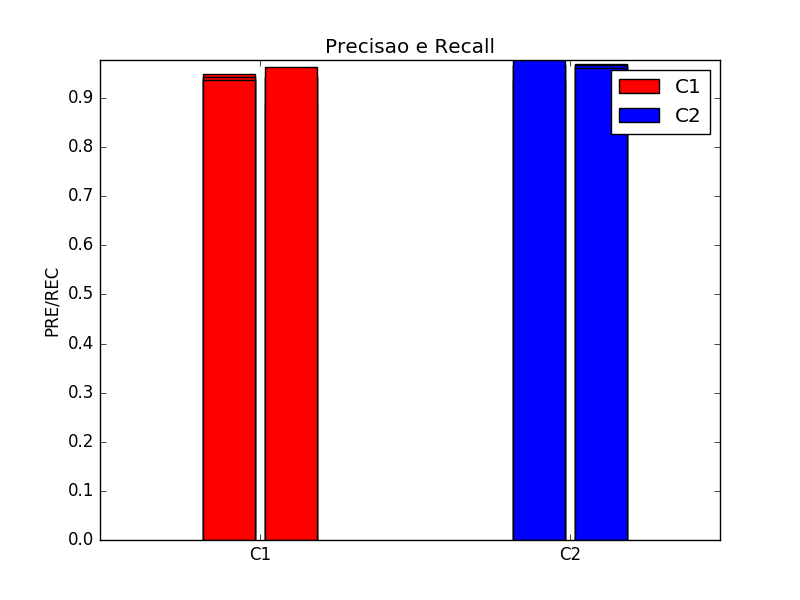
\includegraphics[width=\linewidth]{../img/perc_rec.png}
  \captionof{figure}{Precisão e Recall}
  \label{fig:percep}
\end{figure}%

\end{columns}
\end{frame}


\begin{frame}
\frametitle{Perceptron de Múltiplas Camadas}
\begin{itemize}
  \item asdxf
\end{itemize}
\end{frame}

\begin{frame}[fragile] % Need to use the fragile option when verbatim is used in the slide
\frametitle{Perceptron de Múltiplas Camadas - Implementação}
\begin{block}{Scikit Learn}
\begin{verbatim}
class sklearn.neural_network.MLPClassifier
(hidden_layer_sizes=(100, ), activation='relu',
 solver='adam', alpha=0.0001, batch_size='auto',
 learning_rate='constant', learning_rate_init=0.001,
 power_t=0.5, max_iter=200, shuffle=True, 
random_state=None, tol=0.0001, verbose=False,
 warm_start=False, momentum=0.9, nesterovs_momentum=True,
 early_stopping=False, validation_fraction=0.1,
 beta_1=0.9, beta_2=0.999, epsilon=1e-08)
\end{verbatim}
\end{block}

\end{frame}

\begin{frame}
\frametitle{Perceptron de Múltiplas Camadas - Resultados}
\textbf{Avaliação dos resultados}
\begin{columns}[c] 
\column{.45\textwidth} % Left column and width
\begin{itemize}
\item ACC = 0.97
\end{itemize}

\begin{table}
\begin{tabular}{l l l}
\toprule
 & \textbf{$\hat{C}_1$ (Predita)} & \textbf{$\hat{C}_2$(Predita)}\\
\midrule
$C_1$ & 20.20&1.00\\
$C_2$ & 0.40&35.30\\ 
\bottomrule
\end{tabular}
\caption{Matriz de confusão}
\end{table}


\column{.5\textwidth} % Right column and width
\begin{figure}[H]
\centering
  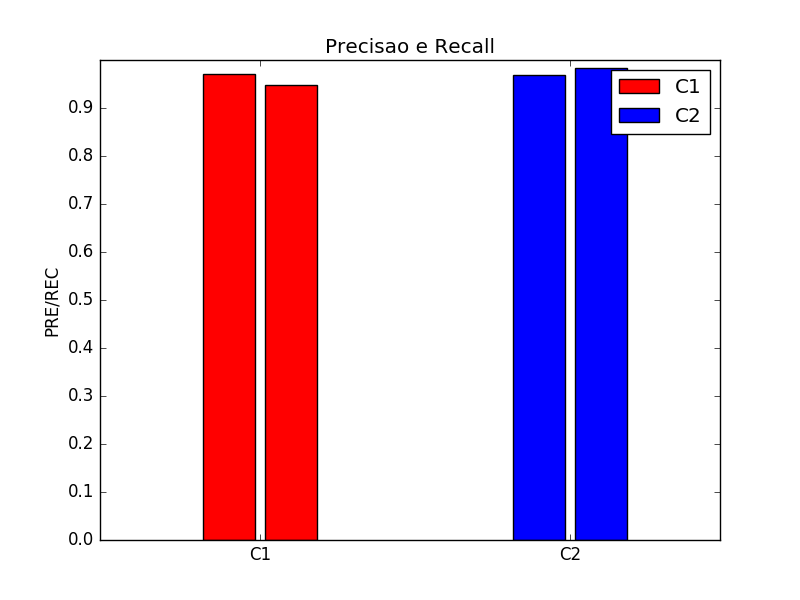
\includegraphics[width=\linewidth]{../img/mlp_rec.png}
  \captionof{figure}{Precisão e Recall}
  \label{fig:percep}
\end{figure}%

\end{columns}

\end{frame}

\end{document} 